\section{Design}
\label{sec:design}


In this section, we first describe a basic protocol that achieves TAP privacy
and action service privacy, and then describe an extension that achieves TAP
anonymity.

\subsection{The basic protocol}

\begin{figure}
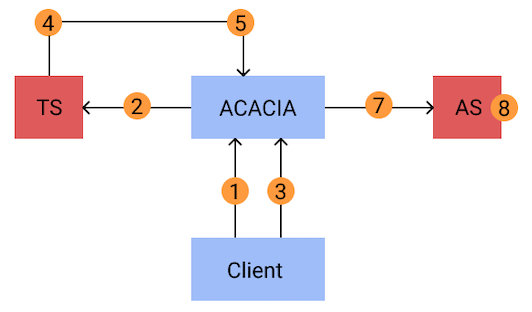
\includegraphics[width=8cm]{/Users/veronikakitsul/Desktop/TAP-research/graphics/ACACIA.png}
\caption{Basic protocol scheme. (1) - (2) (3) (4) (5) (6) (7) (8)}
\end{figure}

\paragraph{Setup.}
Each trigger service $t \in [T]$ has a key pair $(\skt_t, \pkt_t)$ and each
action service $a \in [A]$ has a key pair $(\ska_a, \pka_a)$.

\paragraph{Recipe installation.}
To set up a recipe on the TAP, the client specifies the following through the
trusted mobile client:
\begin{itemize}
  \item a trigger service $t \in [T]$, a predicate $p \in \mathbf{P}_t$, and a
    trigger constant $c_t \in \mathcal{C}$;
  \item an action service $a \in [A]$, a transformation $f \in \mathbf{T}_a$,
    and an action constant $c_a \in \mathcal{C}$.
\end{itemize}
The mobile client encrypts and sends the predicate $p$ and trigger constant
$c_t$ to the trigger service $t$ using its public key $\pkt_t$. The trigger
service can decrypt this information using its secret key $\skt_t$.

%\begin{enumerate}
%  \item The client sends the following to the TAP: $(t, p, \ct_t)$ and $(a, f)$,
%    where $\ct_t = \enc(\skt_t, c_t)$.
%  \item The TAP forwards $(p, \ct_t)$ to $t$ and negotiates the necessary OAuth
%    tokens with $a$ for running the recipe.
%\end{enumerate}

\paragraph{Garbled circuit generation.}
Since the trusted mobile client cannot send the action constant $c_a$ to the TAP
in the clear for the computation of $f(x_t, c_a)$, the client periodically
generates garbled circuits for the transformation, which then allows $y = f(x_t,
c_a)$ to be computed without the TAP learning $x_t$ or $c_a$. Importantly, the
output $y$ must be encrypted under the action service's public key $\pka_a$, so
that the action service can decrypt the result using its secret key $\ska_a$.

\paragraph{Recipe execution.}
When the trigger service $t$ receives trigger data $x_t \in \mathcal{X}$, it
executes $p(x_t, c_t)$. If the result is 1, it encodes its input $x_t$ to the
TAP in order to compute $f(x_t, c_a)$ using MPC. Otherwise, the trigger service
sends nothing. When the TAP receives the encoded input, it computes $f(x_t,
c_a)$ using MPC and sends the encrypted result to the action service $a$. The
action service $a$ decrypts to recover the action data, and then performs its
action.

\subsection{Anonymity extension}

\begin{figure}
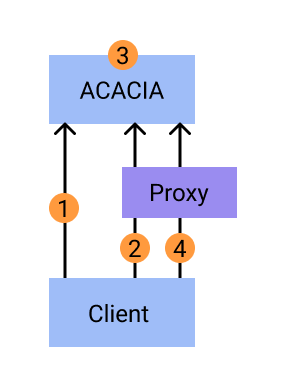
\includegraphics[height=8cm]{/Users/veronikakitsul/Desktop/TAP-research/graphics/Proxy1.png}
\caption{Basic protocol scheme. (1) - (2) (3) (4) (5) (6) (7) (8)}
\end{figure}

\paragraph{Anonymous recipe installation.} In order to achieve TAP anonymity,
clients first need a way to install recipes anonymously. The main cryptographic
tool we use is an anonymous token. This allows the TAP to issue tokens that
authorize clients to install recipes. When the client later wishes to install a
recipe anonymously, it does so through an anonymity proxy (e.g., Tor) by
presenting the required recipe installation data along with an anonymous
token. Importantly, the redemption of this token cannot be linked backed to its
issuance, so the TAP cannot learn who it initially issued this token to.

\paragraph{Anonymous garbled circuit generation.}
Similar to anonymous recipe installation, clients upload garbled circuits
anonymously through an anonymity proxy and present an anonymous token that
authorizes the client to upload garbled circuits for a particular recipe.

\paragraph{Anonymous recipe execution.} Recipes execute as in the basic
protocol, since the garbled circuits for MPC are already set up on the TAP.

\subsection{Security analysis}

Here, we give an informal security analysis and defer the formal analysis to
later.

\paragraph{TAP privacy.} For TAP privacy, the TAP should not learn $x_t$, $c_t$,
$c_a$, or the result of $f(x_t, c_a)$:
\begin{itemize}
  \item The TAP does not learn $c_t$, since it is encrypted to the trigger
    service.
  \item The TAP does not learn $x_t$ or $c_a$, since $f(x_t, c_a)$ is executed
    using MPC.
  \item The TAP does not learn the result of $f(x_t, c_a)$, since it is
    encrypted to the action service.
\end{itemize}

\paragraph{Action service privacy.} For action service privacy, the action
service should not learn $x_t$, except what can be inferred from the output of
$f(x_t, c_a)$.
\begin{itemize}
  \item The action service does not learn $x_t$, except what can be inferred
    from the output of $f(x_t, c_a)$, since the transformation is executed using
    MPC.
\end{itemize}

\paragraph{TAP anonymity.} For TAP anonymity, the TAP should not be able to link
installed rules to a particular client.
\begin{itemize}
  \item The TAP cannot link installed rules to a particular client, since recipe
    installation and garbled circuit uploads are done using an anonymity proxy
    and are authorized via anonymous tokens.
\end{itemize}

\iffalse
Things we want to hide from the TAP (in order from most important to least
important):
\begin{itemize}[leftmargin=*]
  \item inputs to the applet (sleep duration),
  \item outputs to the action service (the reminder),
  \item the applet semantics (``If sleep is under a target duration, then add a
    reminder to Google Calendar.''), and
  \item the services (Fitbit and Google Calendar).
\end{itemize}\bigskip

Unavoidable leakage that we might be able to leverage:
\begin{itemize}[leftmargin=*]
  \item The trigger service (Fitbit) already knows the inputs to the applet
    (sleep duration).
  \item The action service (Google Calendar) will see the outputs (the
    reminder).
\end{itemize}\bigskip

How to hide the inputs to the applet?
\begin{itemize}[leftmargin=*]
  \item \emph{Multi-party computation (MPC).} The trigger service and TAP can
    run a 2-PC to hide the inputs from the TAP.
    \begin{itemize}
      \item Pros: General-purpose (can compute any function over the inputs) and
        achieves the desired notion of privacy (learns nothing about inputs
        except what can be inferred from output)
      \item Cons: Complicated and expensive, may require the client to be online
        periodically, doesn't seem like the right tool for the job since the TAP
        has no inputs, can't hide applet semantics from the TAP
    \end{itemize}
  \item \emph{Private function evaluation (PFE).} PFE hides both the input and
    the function being computed~\cite{DBLP:conf/eurocrypt/MohasselS13}, though
    it might be very slow.
  \item \emph{Trigger service computation.} The trigger service computes the
    conditional (i.e., ``If sleep is under a target duration'').
    \begin{itemize}
      \item Pros: Simple and efficient, achieves the desired notation of
        privacy, maybe still possible to hide applet semantics from the TAP
      \item Cons: Requires trigger service to do work (significant change from
        how things are done today)
    \end{itemize}
\end{itemize}\bigskip

How to hide the outputs of the applet?
\begin{itemize}[leftmargin=*]
  \item \emph{Encrypt to action service.} Need to know more about how actions
    work. Are they static (i.e., send message to action service)? Are they
    dynamic (i.e., inject part of input into message to action service)?
    \begin{itemize}
      \item Note: This is expensive to do in MPC, but easy otherwise (each
        action service has public key, and client installs action rule with TAP
        that encrypts the message to the action service).
    \end{itemize}
\end{itemize}\bigskip

How to hide the applet semantics?
\begin{itemize}[leftmargin=*]
  \item \emph{Trigger service talks to action service directly.} Trigger service
    learns actions service, have to give OAuth tokens to trigger service (some
    trigger services might be sketchy), trigger service has to do more work.
  \item \emph{Trigger service computation + encrypt to action service.}  Client
    generates fresh key pair and installs public key with trigger service and
    secret key with action service. Trigger service encrypts true/false to
    action service, and proxies through TAP. Action service decrypts result,
    uses oblivious transfer to retrieve action output.
\end{itemize}\bigskip

How to hide the services?
\begin{itemize}[leftmargin=*]
  \item This is probably too hard (probably have to add proxies).
\end{itemize}\bigskip

\paragraph{Protocol flow.}
The client installs an applet as follows:
\begin{enumerate}[leftmargin=*]
\item The client generates a key pair $(\sk, \pk)$.
\item The client sends $\sk$ to the action service and $\pk$ to the trigger
  service.
\item On the trigger service, the client installs a rule with an action
  encrypted to the action service.
\item On the TAP, the client configures forwarding/polling rules between trigger
  service and action service.
\end{enumerate}
Applets run as follows:
\begin{enumerate}[leftmargin=*]
\item The trigger service evaluates the rule, and encrypts the resulting bit to
  the action service. If the result is 1, then the trigger service sends the
  encrypted action to the TAP. Otherwise, if the result is 0, then the trigger
  service sends an encryption of zeros to the TAP.
\item The TAP forwards the message to the action service.
\item The action service decrypts the message and executes the action if valid.
\end{enumerate}

\bigskip
Questions to think about:
\begin{itemize}[leftmargin=*]
\item How to add integrity?
\item Xiangchang Mi et al. paper creates a service on IFTTT to see the interaction from both channels,
while testing we would need to the same thing and see how much we can learn about the recipe or
other things.
\item same paper found the delays between triggers and actions because of IFTTT's long polling interval (sometimes up to 15min, usually 1-2min) -- try to see if we can find what is the IFTTT's polling interval and if we can improve it without traffic overload?
\item same paper: when multiple applets run sequentially and concurrently, they form explicit and implicit infinite loops, wasting or damaging devices. How can we improve this?
\end{itemize}
\fi
